\documentclass[border=0.2cm]{standalone}

\usepackage{../mthesis-img} 
 
\begin{document}
 
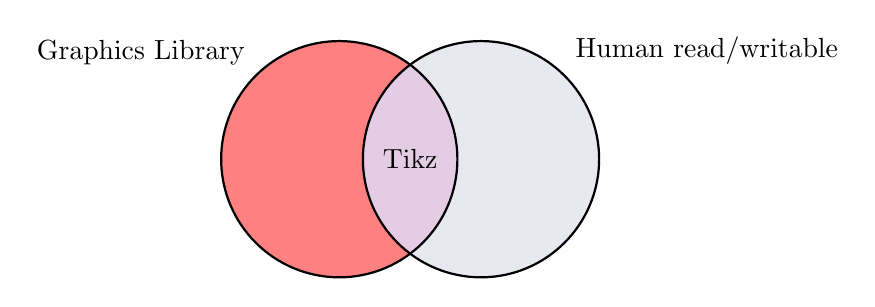
\begin{tikzpicture}[thick,
    set/.style = {circle,
        minimum size = 3cm}]
 
% Set A
\node[set,label={135:Graphics Library},fill=Red!50] (A) at (0,0) {};
 
% Set B
\node[set,label={45:Human read/writable},fill=MidnightBlue!10] (B) at (1.8,0) {};
 
% Intersection
\begin{scope}
    \clip (0,0) circle(1.5cm);
    \clip (1.8,0) circle(1.5cm);
    \fill[Purple!20](0,0) circle(1.5cm);
\end{scope}
 
% Circles outline
\draw (0,0) circle(1.5cm);
\draw (1.8,0) circle(1.5cm);
 
% Set intersection label
\node at (0.9,0) {Tikz};
 
\end{tikzpicture}
 
\end{document}